\documentclass[a4paper,oneside,12pt]{report}
\usepackage{styles/fbe_tez}
\usepackage[utf8x]{inputenc} % To use Unicode (e.g. Turkish) characters
\usepackage{amsmath, amsthm} % Some extra symbols
\usepackage[bottom]{footmisc}
\usepackage{cite}
\usepackage{graphicx}
\usepackage{longtable}
\usepackage{float}
\usepackage{multirow}
\usepackage{algorithm}
\usepackage{algorithmic}
\usepackage{array}
\usepackage{amssymb,bm,cite,graphicx, fixmath, texdraw}
\usepackage{epsfig}
\usepackage{epstopdf}
\usepackage{amsmath}
\usepackage{notoccite}
\usepackage{subcaption}
\usepackage{tabu}

\interdisplaylinepenalty=2500
\hyphenation{lists} \makeatletter

\newcommand{\field}[1]{\mathbb{#1} }
\newcommand{\beq}{\begin{equation} \setlength\abovedisplayskip{5pt} 
\setlength\belowdisplayskip{5pt}}
\newcommand{\eeq}{\end{equation}}
\newcommand{\bea}{\begin{eqnarray}}
\newcommand{\eea}{\end{eqnarray}}
\newcommand{\defn}{\stackrel{\triangle}{=}}
\newcommand{\nn}{\nonumber}
\newcommand{\nnl}{\nonumber \\}
\renewcommand{\theequation}{\arabic{equation}}
\renewcommand{\labelenumi}{(\roman{enumi})}

\DeclareMathOperator*{\argmin}{arg\,min}
\DeclareMathOperator*{\argmax}{arg\,max}

\def\ifundefined{\@ifundefined}
\def\bfat{\left[ \begin{array}}
\def\emat{\end{array} \right]}
\def\bfatt{\left\{ \begin{array}}
\def\ematt{\end{array} \right.}
\def\bset{\left\{ \begin{array}}
\def\eset{\end{array} \right\}}
\def\bpar{\left( \begin{array}}
\def\epar{\end{array} \right)}

\graphicspath{{figures/}} % Graphics will be here

\newtheorem{thm}{Theorem}[chapter]
\newtheorem{prop}[thm]{Proposition}
\newtheorem{lem}[thm]{Lemma}
\newtheorem{cor}[thm]{Corollary}

\numberwithin{equation}{chapter}

% BEGIN OF DOCS
\begin{document}
\pagenumbering{roman}


% CONTENTS AND LIST OF FIG AND TABLE PAGES
\tableofcontents

\pagenumbering{arabic}

%#####
% START OF THEORY
\newcommand{\vecthreeBF}[1]{\vec{\textbf{#1}}}
\newcommand{\vecthree}[1]{\vec{#1}}
\newcommand{\vecNum}[3]{(#1, #2, #3)}

\newcommand{\parDeriv}[2]{\frac{\partial #1}{\partial #2}}
\newcommand{\parDerivS}[2]{\frac{\partial^2 #1}{\partial #2^2}}
\newcommand{\derivS}[2]{\frac{d^2 #1}{d#2^2}}

\newcommand{\dotProdBF}[2]{\vecthreeBF{#1} \cdot \vecthreeBF{#2}}
\newcommand{\dotProd}[2]{\vecthree{#1} \cdot \vecthree{#2}}

\newcommand{\crossProdBF}[2]{\vecthreeBF{#1} \times \vecthreeBF{#2}}
\newcommand{\crossProd}[2]{\vecthree{#1} \times \vecthree{#2}}

\newcommand{\e}{$\textbf{e}^-$ }
\newcommand{\egun}{$\textbf{e}^-$-gun }
\newcommand{\eB}{$\textbf{e}^-$ - $\vecthreeBF{B}$ }
\newcommand{\eE}{$\textbf{e}^-$ - $\vecthreeBF{E}$ }
\newcommand{\eEM}{$\textbf{e}^-$ - \textbf{EM} }
\newcommand{\ee}{$\textbf{e}^-$ - $\textbf{e}^-$ }


\newcommand{\fromeq}[1]{\textit{equation \ref{eq:#1}}}
\newcommand{\fromeqs}[2]{\textit{equations \ref{eq:#1} and \ref{eq:#2}}}
\newcommand{\fromeqsth}[3]{\textit{equations \ref{eq:#1}, \ref{eq:#2} and \ref{eq:#3}}}
\newcommand{\fromeqsf}[4]{\textit{equations \ref{eq:#1}, \ref{eq:#2}, \ref{eq:#3} and \ref{eq:#4}}}

\newcommand{\fromfig}[1]{\textit{figure \ref{fig:#1}}}
\newcommand{\fromfigs}[2]{\textit{figures \ref{fig:#1} and \ref{fig:#2}}}
\newcommand{\fromfigf}[4]{\textit{figures \ref{fig:#1}, \ref{fig:#2}, \ref{fig:#3} and \ref{fig:#4}}}

\newcommand{\fromsec}[1]{\textit{section \ref{sec:#1}}}
\newcommand{\fromsecs}[2]{\textit{sections \ref{sec:#1} and \ref{sec:#2}}}

\newcommand{\fromapp}[1]{\textit{Appendix \ref{appendix:#1}}}

\newcommand{\fromtab}[1]{\textit{Table \ref{tab:#1}}}
\newcommand{\fromtabs}[2]{\textit{Tables \ref{tab:#1} and \ref{tab:#2}}}

\chapter{THEORY}

% START OF PRODUCTION

\chapter{PRODUCTION}
% Start of final.tex
\section{Final Design} \label{sec:final_design}

As discussed before, production efforts of a rhodotron type accelerator is still ongoing in KAHVELab.
This accelerator will be used at $f=107.5$MHz $P=50-100$kW. 
In the following figures, rendered visuals of the final design from a CAD software can be observed.


\newpage


% Start of techd.tex
\section{Technical Drawing}

Technical drawings of the design mentioned in \fromsec{final_design} can be found in following figures:

\begin{figure}[H]
    \centering
    \includegraphics[width=1\linewidth]{./figures/teknikcizim/altgovdeteknikresim.pdf}
    \caption{Technical drawing of bottom part cross section of the cavity. \\ Courtesy of Mr. Sinan Öz}
\end{figure}

\begin{figure}
    \centering
    \includegraphics[angle=270,origin=c, width=.98\linewidth]{./figures/teknikcizim/Rho-A1.0.00.pdf}
    \caption{Technical drawing of the rhodotron cavity. \\ Courtesy of Mr. Sinan Öz}
\end{figure}

\begin{figure}
    \centering
    \includegraphics[angle=270,origin=c, width=.98\linewidth]{./figures/teknikcizim/Rho-A1.1.00.pdf}
    \caption{Technical drawing of upper part of the cavity. \\ Courtesy of Mr. Sinan Öz}
\end{figure}

\begin{figure}
    \centering
    \includegraphics[angle=270,origin=c, width=.98\linewidth]{./figures/teknikcizim/Rho-A1.2.00.pdf}
    \caption{Technical drawing of middle part of the cavity which contains the beam line. \\ Courtesy of Mr. Sinan Öz}
\end{figure}

\begin{figure}
    \centering
    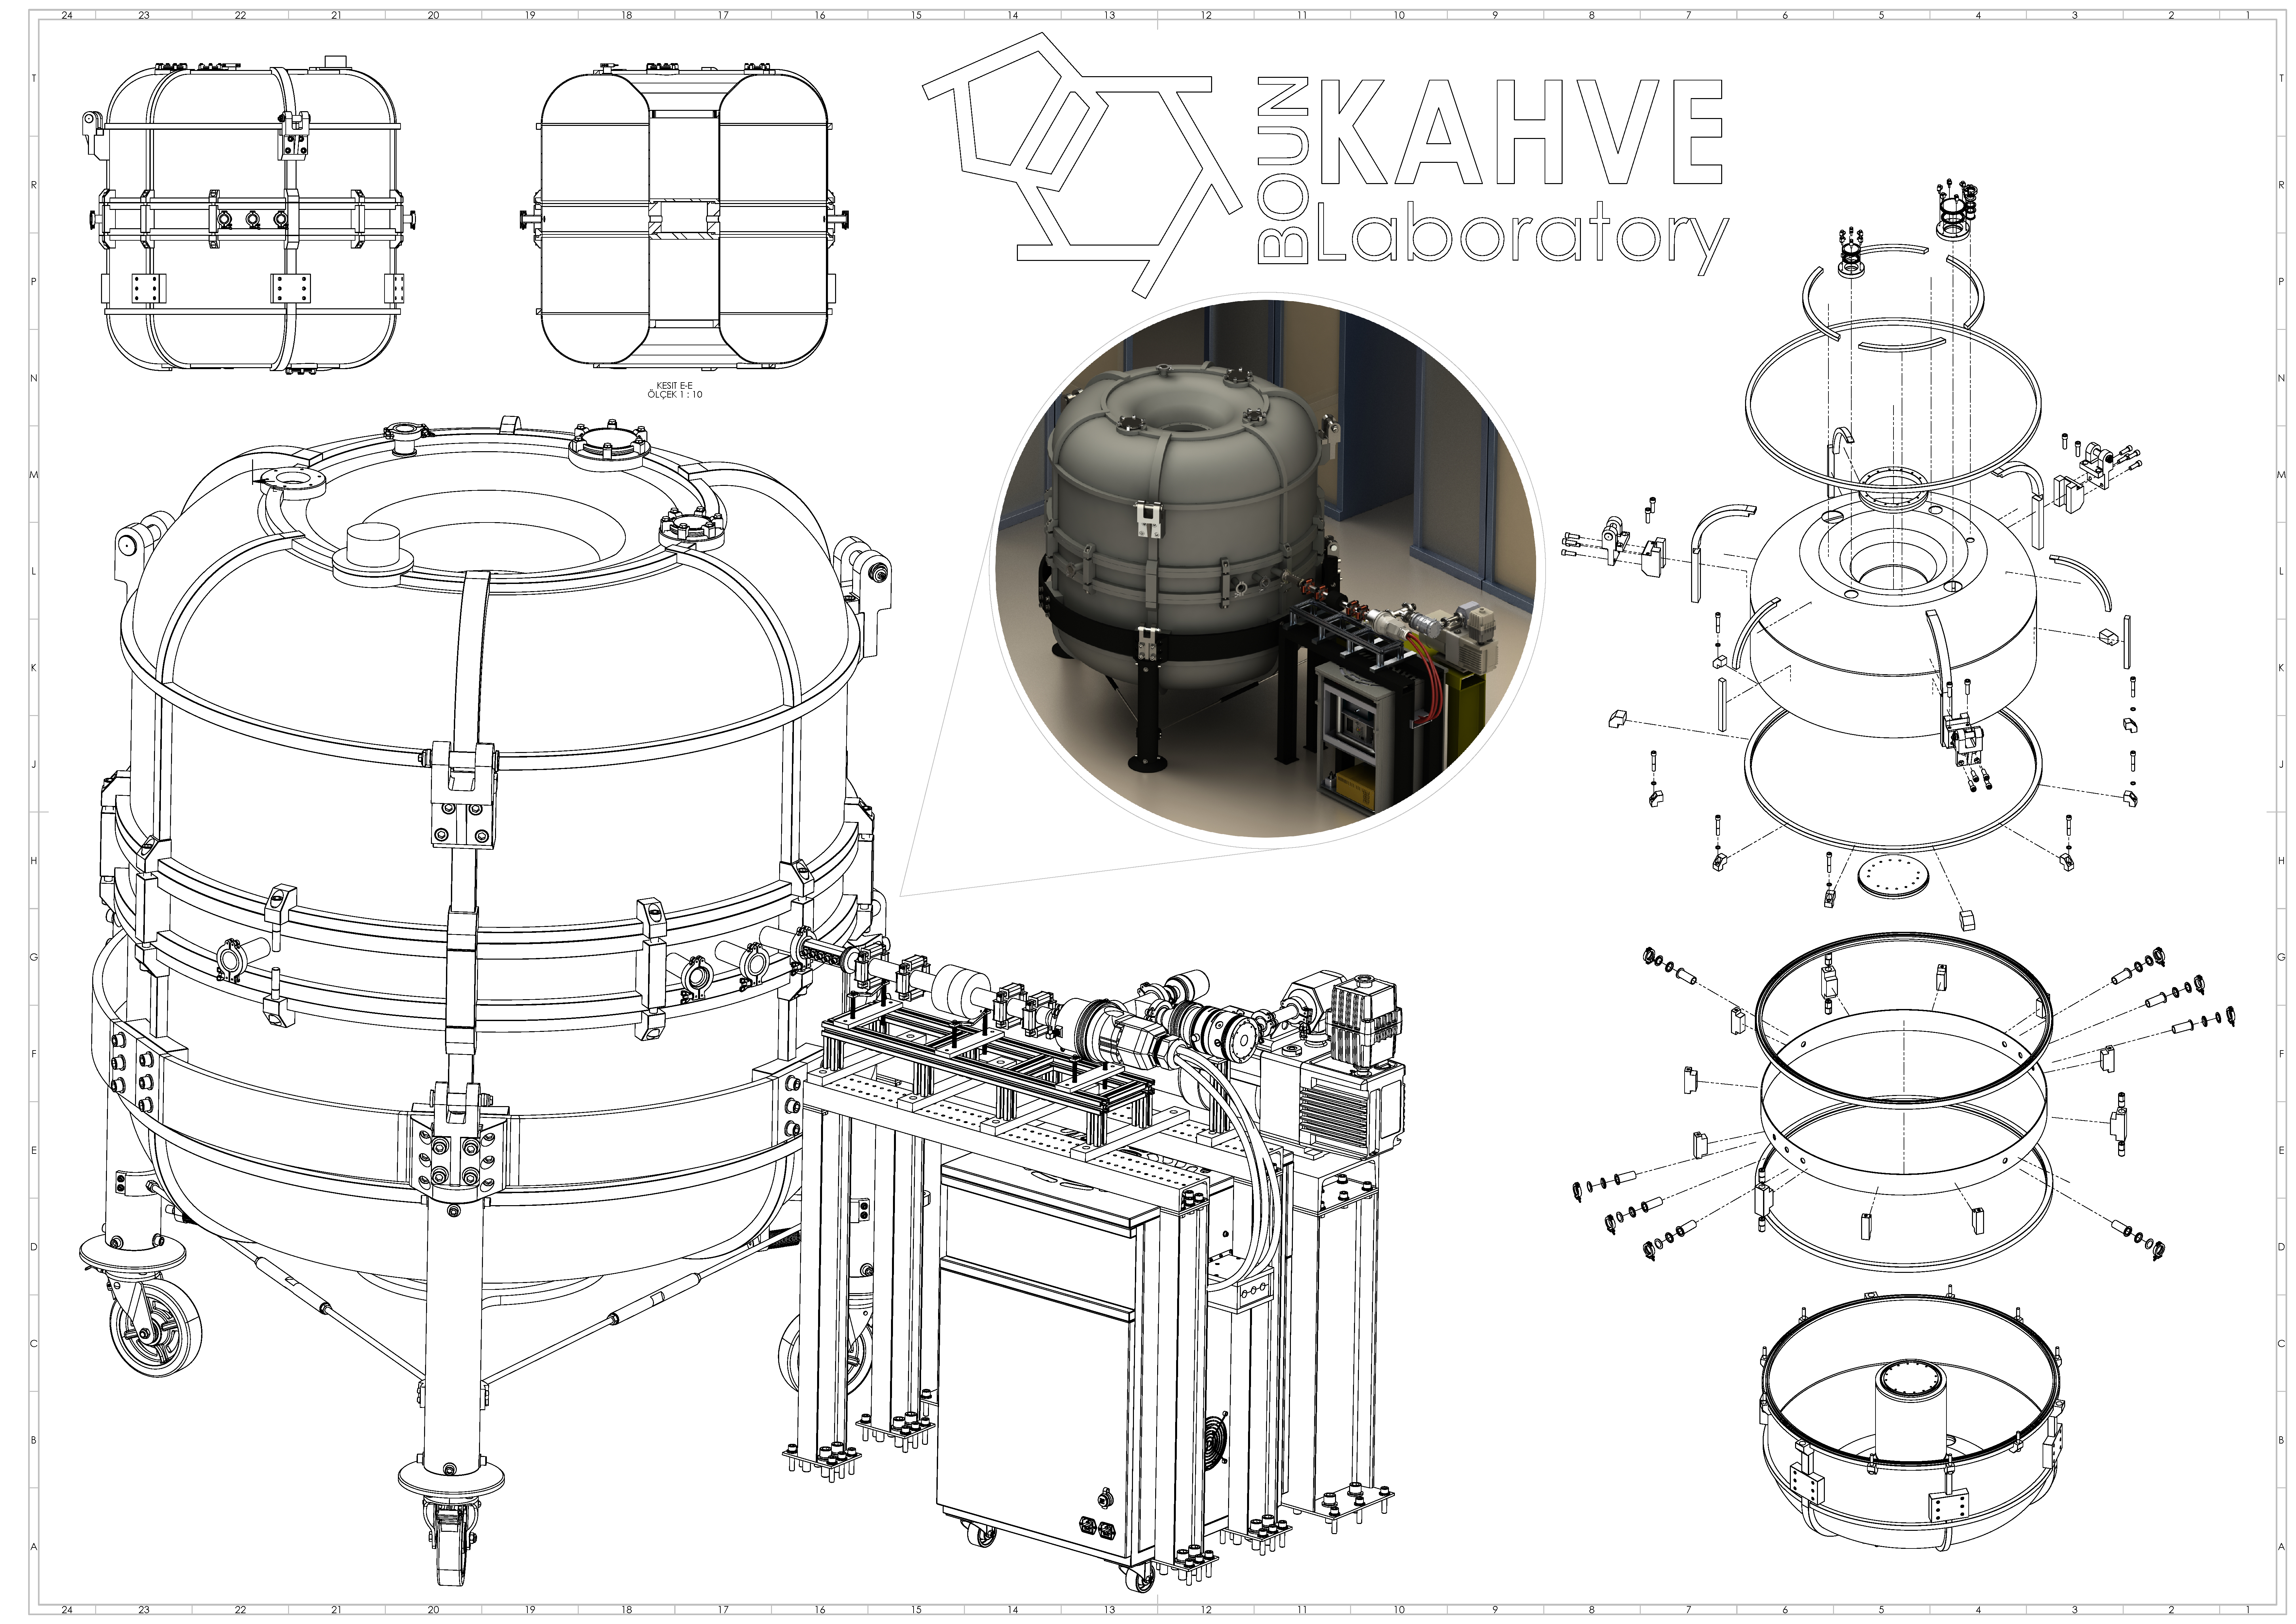
\includegraphics[angle=270,origin=c, width=\linewidth]{./figures/teknikcizim/Rhodotron Elektron Hizlandirici Sistemi.pdf}
    \caption{Technical drawing of middle part of the cavity which contains the beam line. \\ Courtesy of Mr. Sinan Öz}
\end{figure}



\newpage


% Start of mani.tex
\section{Manifacturing}

Manifacturing of the rhodotron cavity has been ongoing, planned to be completed in the following months.

The cavity itself was manifactured as 5 main parts, using 5mm thick stainless steel sheet. 

Elastic version of the 304, 304L was chosen to be the production material for ease of bending.
These sheets were then pressed to achieve the shapes of the parts. 
Several flanges were then machined, including
\begin{itemize}
    \item $4.5$in EIA RF flange for RF input
    \item ISO100-KF vacuum connector flanges for vacuum pumps
    \item ISO-63 KF flange for probe insertion
    \item KF40 flanges for beam line vacuum gauges
\end{itemize}

After desired shapes were produced inside surface of the sheets were polished with 2000 grits. 
304 stainless steel sheet bars of different sizes were then added by 
TIG welding to achieve pressure resistance.

Because the main body of the cavity was 5mm thick and 304L was used, deformations on cylinderical symmetry were encountered. 
This problem was solved by welding 6 10mm thick toroidal sheets between the coaxial cylinders, 
which would be removed after the heat treatment.

\begin{figure}
    %\captionsetup[subfigure]{justification=centering}
    %\captionsetup{justification=centering}
    \centering
    \begin{subfigure}{.5\textwidth}
      \centering
      \includegraphics[width=.96\linewidth]{./figures/manif/polish/rhodo_bottom_unpolished_cropped.jpeg}
      \caption{Bottom part of the cavity while polishing.}
    \end{subfigure}%
    \centering
    \begin{subfigure}{.5\textwidth}
      \centering
      \includegraphics[width=.96\linewidth]{./figures/manif/polish/rhodo_upper_polished_cropped.jpeg}
      \caption{Top part of the cavity after polishing.}
    \end{subfigure}
    \caption{Polishing of the inner surface of cavity.}
    \label{fig:manif_polishing}
\end{figure}


\begin{figure}
    %\captionsetup[subfigure]{justification=centering}
    %\captionsetup{justification=centering}
    \centering
    \begin{subfigure}{.5\textwidth}
      \centering
      \includegraphics[width=.96\linewidth]{./figures/manif/toroidal_sheets/rhodo_bottom_cropped.jpeg}
      \caption{Bottom part of the cavity with the exposed beam line in inner cylinder.}
    \end{subfigure}%
    \centering
    \begin{subfigure}{.5\textwidth}
      \centering
      \includegraphics[width=.96\linewidth]{./figures/manif/toroidal_sheets/rhodo_middle_toroidal_sheets_welded_cropped.jpeg}
      \caption{Bottom part of the cavity with the beam line assembled.}
    \end{subfigure}
    \caption{Deformation prevention measure, 10 mm thick toroidal sheets.}
    \label{fig:manif_toroidal_sheets}
\end{figure}

\begin{figure}
    %\captionsetup{justification=centering}
    \centering
    \includegraphics[width=.8\linewidth]{./figures/manif/welding/rhodo_middle_sheetbars_cropped.jpeg}
    \caption{Welded sheet bars.}
\end{figure}

\begin{figure}
    %\captionsetup{justification=centering}
    \centering
    \includegraphics[width=.7\linewidth]{./figures/manif/toroidal_sheets/rhodo_middle_only_cropped.jpeg}
    \caption{Middle part of the cavity containing the beam line.}
\end{figure}


\begin{figure}
    %\captionsetup[subfigure]{justification=centering}
    %\captionsetup{justification=centering}
    \centering
    \begin{subfigure}{.5\textwidth}
      \centering
      \includegraphics[width=.96\linewidth]{./figures/manif/welding/rhodo_assembled_welding_cropped.jpeg}
      \caption{Welding sheet bars.}
    \end{subfigure}%
    \centering
    \begin{subfigure}{.5\textwidth}
      \centering
      \includegraphics[width=.96\linewidth]{./figures/manif/welding/rhodo_middle_welding_toroidal_sheets_cropped.jpeg}
      \caption{Welding toroidal sheets.}
    \end{subfigure}
    \caption{TIG welding.}
    \label{fig:manif_welding}
\end{figure}

\begin{figure}
    %\captionsetup[subfigure]{justification=centering}
    %\captionsetup{justification=centering}
    \centering
    \begin{subfigure}{.5\textwidth}
      \centering
      \includegraphics[width=.96\linewidth]{./figures/manif/assembled/rhodo_assembled_2_cropped.jpeg}
    \end{subfigure}%
    \centering
    \begin{subfigure}{.5\textwidth}
      \centering
      \includegraphics[width=.96\linewidth]{./figures/manif/assembled/rhodo_assembled_1_cropped.jpeg}
    \end{subfigure}
    \caption{Assembled cavity as the current stage.}
    \label{fig:manif_assembled}
\end{figure}




\newpage


% Start of rf.tex
\section{RF Supply}





% END OF THEORY
%#####
\end{document}
